% This file was created with tikzplotlib v0.10.1.
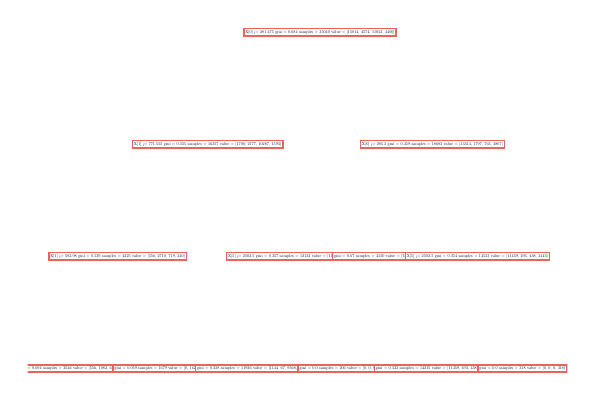
\begin{tikzpicture}

\definecolor{darkgray176}{RGB}{176,176,176}
\definecolor{tomato2369992}{RGB}{236,99,92}

\begin{axis}[
hide x axis,
hide y axis,
tick align=outside,
tick pos=left,
x grid style={darkgray176},
xmin=0, xmax=1,
xtick style={color=black},
y grid style={darkgray176},
ymin=0, ymax=1,
ytick style={color=black}
]
\draw (axis cs:0.0833333333333333,0.125) node[
  scale=0.151685618250733,
  fill=white,
  draw=tomato2369992,
  line width=0.6pt,
  inner sep=3.6pt,
  text=black,
  rotate=0.0,
  align=center
]{gini = 0.694
samples = 2546
value = [556, 1082, 668, 240]};
\draw (axis cs:0.25,0.125) node[
  scale=0.151685618250733,
  fill=white,
  draw=tomato2369992,
  line width=0.6pt,
  inner sep=3.6pt,
  text=black,
  rotate=0.0,
  align=center
]{gini = 0.059
samples = 1679
value = [0, 1628, 51, 0]};
\draw (axis cs:0.416666666666667,0.125) node[
  scale=0.151685618250733,
  fill=white,
  draw=tomato2369992,
  line width=0.6pt,
  inner sep=3.6pt,
  text=black,
  rotate=0.0,
  align=center
]{gini = 0.338
samples = 11926
value = [1144, 67, 9568, 1147]};
\draw (axis cs:0.583333333333333,0.125) node[
  scale=0.151685618250733,
  fill=white,
  draw=tomato2369992,
  line width=0.6pt,
  inner sep=3.6pt,
  text=black,
  rotate=0.0,
  align=center
]{gini = 0.0
samples = 206
value = [0, 0, 0, 206]};
\draw (axis cs:0.75,0.125) node[
  scale=0.151685618250733,
  fill=white,
  draw=tomato2369992,
  line width=0.6pt,
  inner sep=3.6pt,
  text=black,
  rotate=0.0,
  align=center
]{gini = 0.332
samples = 14215
value = [11459, 493, 438, 1825]};
\draw (axis cs:0.916666666666667,0.125) node[
  scale=0.151685618250733,
  fill=white,
  draw=tomato2369992,
  line width=0.6pt,
  inner sep=3.6pt,
  text=black,
  rotate=0.0,
  align=center
]{gini = 0.0
samples = 318
value = [0, 0, 0, 318]};
\draw (axis cs:0.166666666666667,0.375) node[
  scale=0.151685618250733,
  fill=white,
  draw=tomato2369992,
  line width=0.6pt,
  inner sep=3.6pt,
  text=black,
  rotate=0.0,
  align=center
]{X[1] <= 582.98
gini = 0.539
samples = 4225
value = [556, 2710, 719, 240]};
\draw (axis cs:0.5,0.375) node[
  scale=0.151685618250733,
  fill=white,
  draw=tomato2369992,
  line width=0.6pt,
  inner sep=3.6pt,
  text=black,
  rotate=0.0,
  align=center
]{X[5] <= 2502.5
gini = 0.357
samples = 12132
value = [1144, 67, 9568, 1353]};
\draw (axis cs:0.666666666666667,0.375) node[
  scale=0.151685618250733,
  fill=white,
  draw=tomato2369992,
  line width=0.6pt,
  inner sep=3.6pt,
  text=black,
  rotate=0.0,
  align=center
]{gini = 0.67
samples = 4150
value = [1855, 1304, 327, 664]};
\draw (axis cs:0.833333333333333,0.375) node[
  scale=0.151685618250733,
  fill=white,
  draw=tomato2369992,
  line width=0.6pt,
  inner sep=3.6pt,
  text=black,
  rotate=0.0,
  align=center
]{X[5] <= 2502.5
gini = 0.354
samples = 14533
value = [11459, 493, 438, 2143]};
\draw (axis cs:0.333333333333333,0.625) node[
  scale=0.151685618250733,
  fill=white,
  draw=tomato2369992,
  line width=0.6pt,
  inner sep=3.6pt,
  text=black,
  rotate=0.0,
  align=center
]{X[1] <= 771.555
gini = 0.555
samples = 16357
value = [1700, 2777, 10287, 1593]};
\draw (axis cs:0.75,0.625) node[
  scale=0.151685618250733,
  fill=white,
  draw=tomato2369992,
  line width=0.6pt,
  inner sep=3.6pt,
  text=black,
  rotate=0.0,
  align=center
]{X[0] <= 285.3
gini = 0.459
samples = 18683
value = [13314, 1797, 765, 2807]};
\draw (axis cs:0.541666666666667,0.875) node[
  scale=0.151685618250733,
  fill=white,
  draw=tomato2369992,
  line width=0.6pt,
  inner sep=3.6pt,
  text=black,
  rotate=0.0,
  align=center
]{X[0] <= 281.475
gini = 0.684
samples = 35040
value = [15014, 4574, 11052, 4400]};
\end{axis}

\end{tikzpicture}
